\documentclass[../background.tex]{subfiles}

\begin{document}

Univariate B-splines are defined as piecewise polynomial curves comprised of linear combinations of B-spline basis functions. The basis functions for B-splines can be produced through a recursion relation utilizing three pieces of information. These are $p$, the polynomial degree, $n$, the number of basis functions and $\Xi$, the so called \textit{knot vector}. 

The knot vector $\Xi$ encodes information about the B-spline's continuity. It is a vector of nondecreasing real numbers $\xi_i$ such that $\xi_i \leq \xi_{i+1}$. To define a B-spline basis, we require $n+p+1$ knots in our knot vector. For our purposes, we will impose two more constraints on the knot vector, that the knot vector is \textit{open} such that the first and last knot are repeated $p+1$ times, and that the knot vector is normalized such that $\xi_1 = 0$ and $\xi_{n+p+1} = 1$.

B-spline basis functions can be computed in a number of ways, but we utilize the Cox-De Boor recursion relation detailed in \cite{de_boor_calculating_1972}. The basis function $N_{i,p}$ is the \textit{ith} basis function of degree $p$. For a detailed explanation of efficient algorithms for computing b-spline bases and their derivatives, we point to any number of books and articles, including \cite{piegl_nurbs_2012,austin_cottrell_isogeometric_2009}.

Multi-dimensional B-spline bases can be built in a tensor product fashion. We can define the multi-index $\mathbf{i} = \{i_1,\dots,i_{d_p}\}$ which defines the index of the basis within the tensor product, and $\mathbf{p} = \{p_1,\dots, p_{d_p}\}$ which defines the polynomial degree in direction $d$. Here, $d_p$ is the dimension of the parametric domain. Then, the basis function in $d_p$ dimensions is defined over the parametric domain with coordinates $\boldsymbol{\xi} = \{\xi_1,\dots, \xi_{d_p}\}$:

\begin{equation}
N_{\mathbf{i},\mathbf{p}}(\boldsymbol{\xi}) = \prod_{d=1}^{d_p} N^d_{i_d, p_d}(\xi_d)
\end{equation}

\begin{figure}[!htbp]
  \centerline{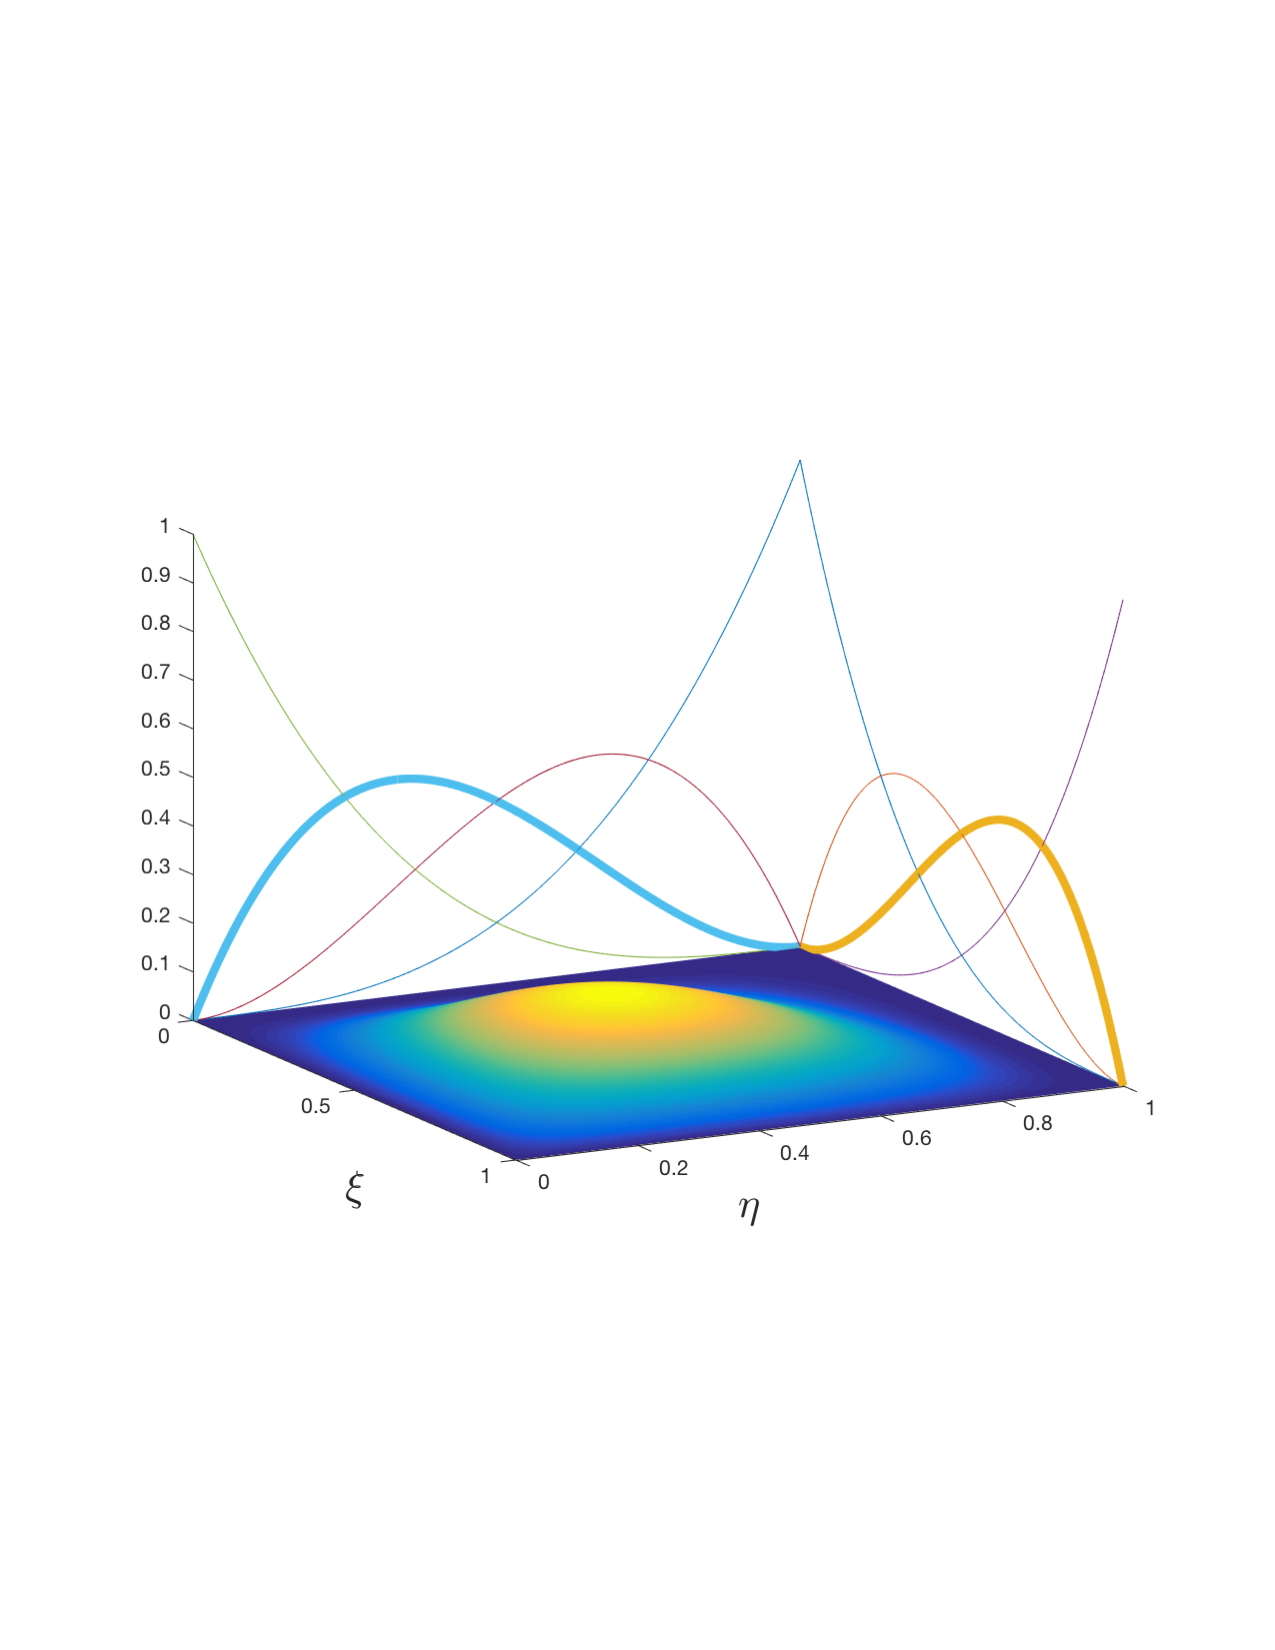
\includegraphics[width=4in]{./figures/2DBSpline_p3}}
  \caption{Typical 2D B-spline basis function}
  \label{fig:BSplines2D}
\end{figure}

We define quantities in terms of B-splines by summing the product of B-spline bases and control variables. For instance, the quantity $\phi(\xi)$ which could be the solution to the advection-diffusion equation over the domain $\Omega$. We approximate $\phi$ with B-splines defined over $\Omega$ and control variables $d^{\phi}_i$:

\begin{equation}
\phi(\xi) = \sum_{i=1}^n d^{\phi}_i N_{i,p}(\boldsymbol{\xi})
\end{equation}

This formulation is useful for simple rectangular domains, and is how we will construct solutions over square domains in this paper, however, we could extend this to more interesting domains by mapping our parametric coordinates $\boldsymbol{\xi}$ to physical coordinates $\mathbf{x}$ via the mapping:

\begin{equation}
\mathbf{x}= \sum_{\mathbf{i}} \mathbf{P}_{\mathbf{i}} N_{\mathbf{i},\mathbf{p}}(\boldsymbol{\xi})
\end{equation}
where $\mathbf{P_i}$ are known as control points, and live in physical space $\mathbf{P_i} \in \mathbb{R}^{d_s}$ where $d_s$ is the dimension of physical space. Setting $d_p = 1$, and $d_s = 3$ allows us to construct curves in 3D space. Similarly, setting $d_p = 2$ and $d_s = 3$ produces surfaces, and so on. 
\end{document}